%%%%%%%%%%%%%%%%%%%%%%%%%%%%%%%%%%%%%%%%%%%%%%%%%%%%%%%%%%%%%%%%%%%%%%%%%%
% The template begins here. Please do not modify the font size from 12 point.

\documentclass[12pt]{article}
\usepackage{phase1}

%%%%%%%%%%%%%%%%%%%%%%%%%%%%%%%%%%%%%%%%%%%%%%%%%%%%%%%%%%%%%
%  PREAMBLE: sets up compiler modes, loads packages, defines macros, etc
%%%%%%%%%%%%%%%%%%%%%%%%%%%%%%%%%%%%%%%%%%%%%%%%%%%%%%%%%%%%%
%%%%%%%%%%%%%%%%%%%%%%%%%%%%%%%%%%%%%%%%%%%%%%%%%%%%%%%%%%%%%
%  PREAMBLE: sets up compiler modes, loads packages, defines macros, etc
%  Steve Rodney, 2012
%%%%%%%%%%%%%%%%%%%%%%%%%%%%%%%%%%%%%%%%%%%%%%%%%%%%%%%%%%%%%


%%%%%%%%%%%%%%%%%%%%
% COMPILER MODES
%%%%%%%%%%%%%%%%%%%%

% Changetext mode : highlight modified text in bold blue font
\newif{\ifchangetext}
\changetextfalse

%% Read in the -options.tex file (generated by the Makefile)
%%  to set the compile-mode options
\InputIfFileExists{\jobname-options}


%%%%%%%%%%%%%%%%%%%%%%%%%%%%%%%
% changetext  mode settings
%%%%%%%%%%%%%%%%%%%%%%%%%%%%%%%
\ifchangetext
  % Changed text is highlighted in bold, blue font 
  \newcommand{\change}[1]{\textcolor{blue}{ \bf #1}}
  \newcommand{\changenote}[1]{\textcolor{blue}{ \bf #1}}
\else
  % Changed text is indistinguishable
  \newcommand{\change}[1]{#1}
  \newcommand{\changenote}[1]{}
\fi


%%%%%%%%%%%%%%%%%%%%
% PACKAGES INCLUDED
%%%%%%%%%%%%%%%%%%%%
\usepackage{deluxetable}  % stand-alone version of AAStex's  deluxetable
\usepackage{journalnames} % Astro Journal abbreviations
\usepackage[svgnames]{xcolor}  % colored text (better than color)
%\usepackage[usenames]{color}  % colored text
\usepackage[linkcolor=blue,citecolor=darkgray,colorlinks=true]{hyperref}
\usepackage{natbib}   % reference citations and bibliography
\usepackage{graphicx}
%\usepackage{enumerate}% enumerated lists
\usepackage{amsmath}  % equations and such
\usepackage{amssymb}  % extended symbols lib
%\usepackage{mathrsfs} % extended math fonts (mathscr)
%\usepackage{breqn}    % automatic line breaks for long equations
%\usepackage{multirow}  % muti-row table cells
%\usepackage{paralist} % inline enumeration (for Table ref lists)
%\usepackage{authblk}
%\usepackage{multicol}
%\usepackage{subfig} % subfloats with independent captions
%\usepackage{subcaption} % subfloats with independent captions
\usepackage{setspace} % switch from double to single spacing
%\usepackage[none]{hyphenat} % Suppress the hyphenating
%\usepackage{verbatim} % verbatim text formatting
%\usepackage{ulem} % for some underlining.
%\usepackage{wrapfig}


%%%%%%%%%%%%%%%%%%%%%%%%%%%%%%%%%%%%%%%%%%%%%%%%%%%
% PDF mode settings : Auto-select eps or pdf figures 
% based  on the compiler used (i.e. latex vs pdflatex)
%%%%%%%%%%%%%%%%%%%%%%%%%%%%%%%%%%%%%%%%%%%%%%%%%%%
\DeclareGraphicsExtensions{.png,.pdf,.jpg}

%%%%%%%%%%%%%%%%%%%%%%%%%%%%%%%
% AUTHOR-DEFINED MACROS
%%%%%%%%%%%%%%%%%%%%%%%%%%%%%%%

% Time delay 
\def\dt{\ensuremath{\Delta t}}
\def\Dl{\ensuremath{D_l}}
\def\Ds{\ensuremath{D_s}}
\def\Dls{\ensuremath{D_{ls}}}

% plus-minus symbols for statistical or systematic errors
\def\pmstat{\ensuremath{\substack{\pm \\ \mbox{\scalebox{0.45}{stat}}}}}
\def\pmsys{\ensuremath{\substack{\pm \\ \mbox{\scalebox{0.45}{sys}}}}}


% prompt Ia fraction
\def\fp{\ensuremath{f_{P}}}
\def\fP{\ensuremath{f_{P}}}

% STARDUST probabilities
\def\pIa{\ensuremath{p_{Ia}}}
\def\pIaz{\ensuremath{p_{Ia,z}}}
\def\pIahost{\ensuremath{p_{Ia,host}}}

% General purpose usefulness:
\newcommand{\etal}{{et al.~}}                                             
\def\eg{{e.g.}}
\def\ie{{i.e.}}
\def\etc{{etc.}}
\newcommand{\lta}{\lesssim}                                               
\newcommand{\gta}{\gtrsim}                                                
\newcommand{\gt}{\gtsim}

% Cosmology:
\def\Om{\ensuremath{\Omega_{\rm m}}}
\def\Ot{\ensuremath{\Omega_{\rm tot}}}
\def\Ob{\ensuremath{\Omega_{\rm b}}}
\def\OL{\ensuremath{\Omega_{\Lambda}}}
\def\Ok{\ensuremath{\Omega_{\rm k}}}
\def\om{\ensuremath{\omega_{\rm m}}}
\def\ob{\ensuremath{\omega_{\rm b}}}
\def\wo{\ensuremath{w_0}}
\def\wa{\ensuremath{w_{\rm a}}}
\def\lcdm{$\Lambda$CDM}
\def\LCDM{$\Lambda$CDM}
\def\wcdm{$w$CDM}
\def\Ho{\ensuremath{H_0}}
\def\DA{\ensuremath{D_A}}
\def\DL{\ensuremath{D_L}}

% Astronomy:
\def\arcsec{\ensuremath{^{\prime\prime}}} 
\def\kms{\ensuremath{{\rm km s}^{-1}}}
\def\hgpcq{\mbox{$h^{-3}$Gpc$^3$}}
\def\hmpcq{\mbox{$h^{-3}$Mpc$^3$}}
\def\perhmpcq{\mbox{$h^{3}$Mpc$^{-3}$}}
\def\hmpc{\mbox{$h^{-1}$Mpc}}
\def\hmpci{\mbox{$h$\,Mpc$^{-1}$}}
\def\mpc{\mbox{Mpc}}
\def\mpci{\mbox{Mpc$^{-1}$}}
\def\mpcq{\mbox{Mpc$^{-3}$}}
\def\Msun{\mbox{M$_{\odot}$}}
\def\Av{\mbox{$A_V$}}
\def\Rv{\mbox{$R_V$}}

% Supernovae : 
\newcommand{\SNuVol}{\ensuremath{10^{-4}~\mbox{yr}^{-1}~\mbox{Mpc}^{-3}~{\mbox{h}_{70}}^{3}}}
\newcommand{\CCSN}{CC\,SN}
\newcommand{\CCSNe}{CC\,SN}
\newcommand{\TNSN}{TN\,SN}
\newcommand{\TNSNe}{TN\,SNe}
\newcommand{\SNIa}{SN\,Ia}
\newcommand{\SNeIa}{SN\,Ia}
\newcommand{\SNRz}{SNR($z$)}
\def\Mch{\mbox{M$_{\rm Ch}$}}
\def\Ni{\ensuremath{^{56}\mbox{Ni}}}
\newcommand{\dmfifteen}{\ensuremath{\Delta\mbox{m}_{15}}}
\newcommand{\deltamfifteen}{\ensuremath{\Delta\mbox{m}_{15}}}
\newcommand{\NM}{\ensuremath{\mbox{\rm N}_{Ia}/\mbox{M}_{*}}}

\def\galsnid{{\it galsnid}}

% SNANA / SALT2
\def\xone{\ensuremath{x_{1}}}
\def\C{\ensuremath{\mathcal{C}}}


% Missions:
\def\HST{{\it HST}}
\def\Hubble{{\it Hubble}}
\def\Hubbles{{\it Hubble's}}
\def\Spitzer{{\it Spitzer}}
\def\Chandra{{\it Chandra}}
\def\Herschel{{\it Herschel}}
\def\XMM{{\it XMM}}


%%%%%%%%%%%%%%%%%%%%%%%%%%%%%%%
% Page Setup 
%%%%%%%%%%%%%%%%%%%%%%%%%%%%%%%
\renewcommand{\topfraction}{0.9}
\renewcommand{\bottomfraction}{0.9}
\renewcommand{\textfraction}{0.1}
\renewcommand{\floatpagefraction}{0.9}
\renewcommand{\dbltopfraction}{0.9}
\renewcommand{\dblfloatpagefraction}{0.9}



%%%%%%%%%%%%%%%%%%%%%%%%%%%%%%%%%%%%
%% Figure placement shortcuts    
%%%%%%%%%%%%%%%%%%%%%%%%%%%%%%%%%%%%

\newcommand{\insertfigwide}[2] {
\begin{figure*}
\begin{center}
\resizebox{\textwidth}{!}{\includegraphics{{#1}}}
\caption{{#2}}
\end{center}
\end{figure*}
}

\newcommand{\insertfigdouble}[3] {
\begin{figure*}
\begin{center}
\resizebox{0.45\textwidth}{!}{\includegraphics{{#1}}}
\resizebox{0.45\textwidth}{!}{\includegraphics{{#2}}}
\figcaption{{#3}}
\end{center}
\end{figure*}
}

\newcommand{\insertfigquad}[5] {
\begin{figure*}
\begin{center}
\resizebox{0.48\textwidth}{!}{\includegraphics{{#1}}}
\resizebox{0.48\textwidth}{!}{\includegraphics{{#2}}}
\resizebox{0.48\textwidth}{!}{\includegraphics{{#3}}}
\resizebox{0.48\textwidth}{!}{\includegraphics{{#4}}}
\figcaption{{#5}}
\end{center}
\end{figure*}
}

\newcommand{\insertfig}[2] {
\begin{figure}
\begin{center}
\resizebox{\columnwidth}{!}{\includegraphics{{#1}}}
\figcaption{{#2}}
\end{center}
\end{figure}
}


\begin{document}

%   1. SCIENTIFIC JUSTIFICATION
%       (see Section 9.1 of the Call for Proposals)
%
%
\justification          % Do not delete this command.
% Enter your scientific justification here. 


The HST archive now holds a deep trove of WFC3-IR imaging on
strong-lensing galaxy clusters at redshifts $z\sim0.5$.  Many of these
clusters have dozens of multiply-imaged background galaxies at
redshifts $1\lesssim z \lesssim 6$, which have been used to produce
well-constrained models of the cluster lensing potential.  When a
supernova (SN) inevitably appears within one of these multiply-imaged
galaxies, it will of course be multiply-imaged itself. 
% {\bf \em With
% this snapshot program, we propose to use WFC3-IR to discover the first
% ever multiply-imaged SN behind a strong lensing galaxy cluster --
% setting a new gold standard for future gravitational lens time delay
% measurements.}
% With even just a single lensed SN
% time delay, we will constrain \Ho\ to better than 6\%
% precision, provide
% powerful new constraints on dark energy parameters, and deliver a unique test
% of systematic biases in other cosmological probes.  Along with the
% accompanying GO program for ToO follow-up, {\bf \em this IR snapshot
% survey will }
 {\bf \em With this snapshot survey, we propose to use WFC3-IR to
discover the first ever multiply-imaged SN behind a strong lensing
galaxy cluster.}  Along with the accompanying GO proposal for ToO
follow-up, {\bf \em this program will set a new gold standard for
future gravitational lens time delay measurements.}  With even just a
single lensed SN time delay, we will constrain \Ho\ to better than 6\%
precision, provide powerful new constraints on dark energy parameters,
and deliver a unique test of systematic biases in other cosmological
probes.


\medskip
\noindent {\bf Time Delay Cosmography}

\noindent As light from a distant source passes through a galaxy cluster,
strong gravitational lensing causes multiple images to appear to the
observer, separated by a time delay 

\vspace{-5mm}
\begin{tabular}{p{5.5cm}r}
% \dt = \frac{\Dl \Ds}{\Dls} ( 1 + z_l ) \phi
{\begin{align}
%\begin{equation}\label{eq:dt}
 %  \dt = \frac{\Dl \Ds}{\Dls} ( 1 + z_l ) \phi
%\end{equation}
  \dt &= \frac{\Dl \Ds}{c\,\Dls} ( 1 + z_L ) \phi \label{eq:dt} \\
  \phi &= \frac{1}{2}(\theta-\beta)^2 - \psi(\theta) \label{eq:phi}
\end{align}}
&
\hspace{1cm}
\raisebox{-30mm}{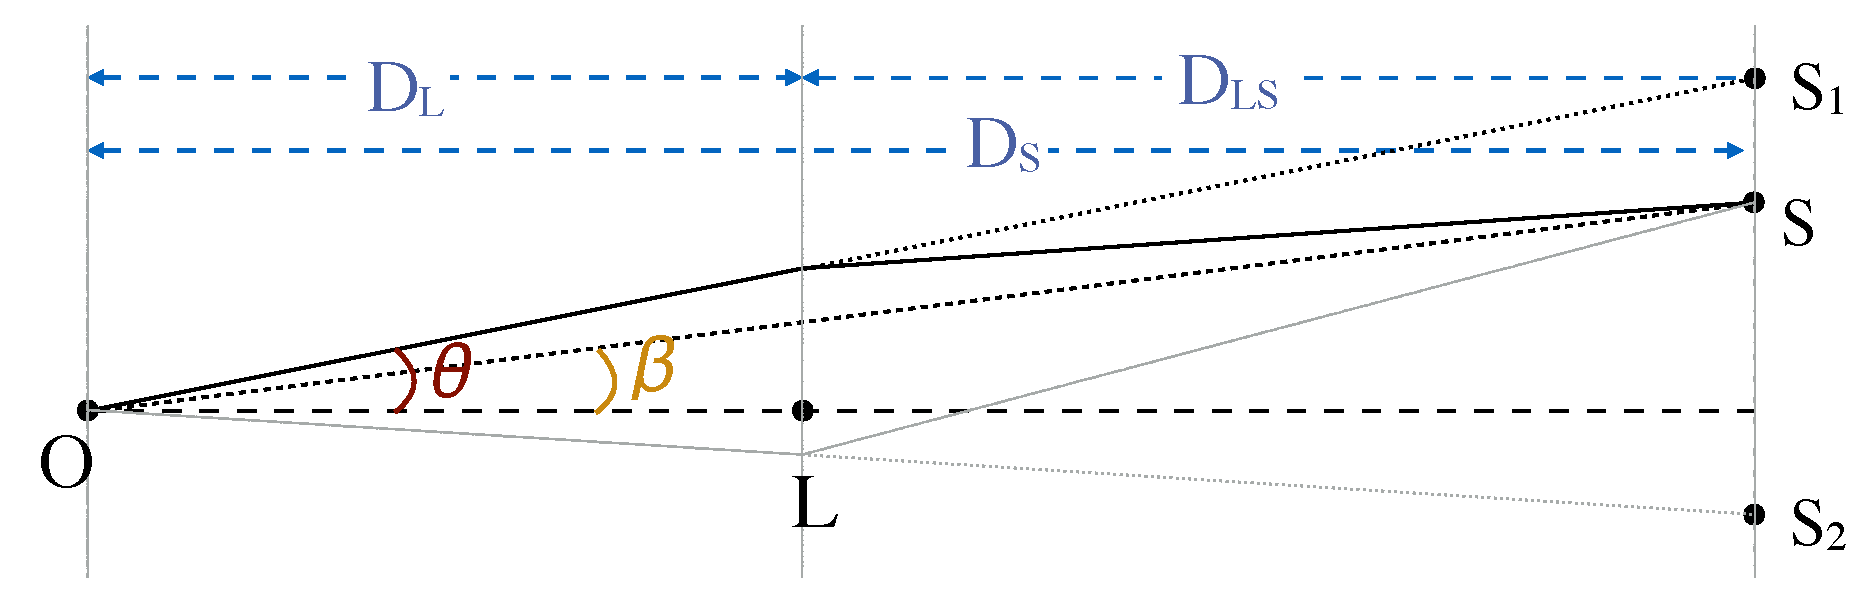
\includegraphics[width=0.5\textwidth]{FIG/lensingGeometry2}}
%\raisebox{-30mm}{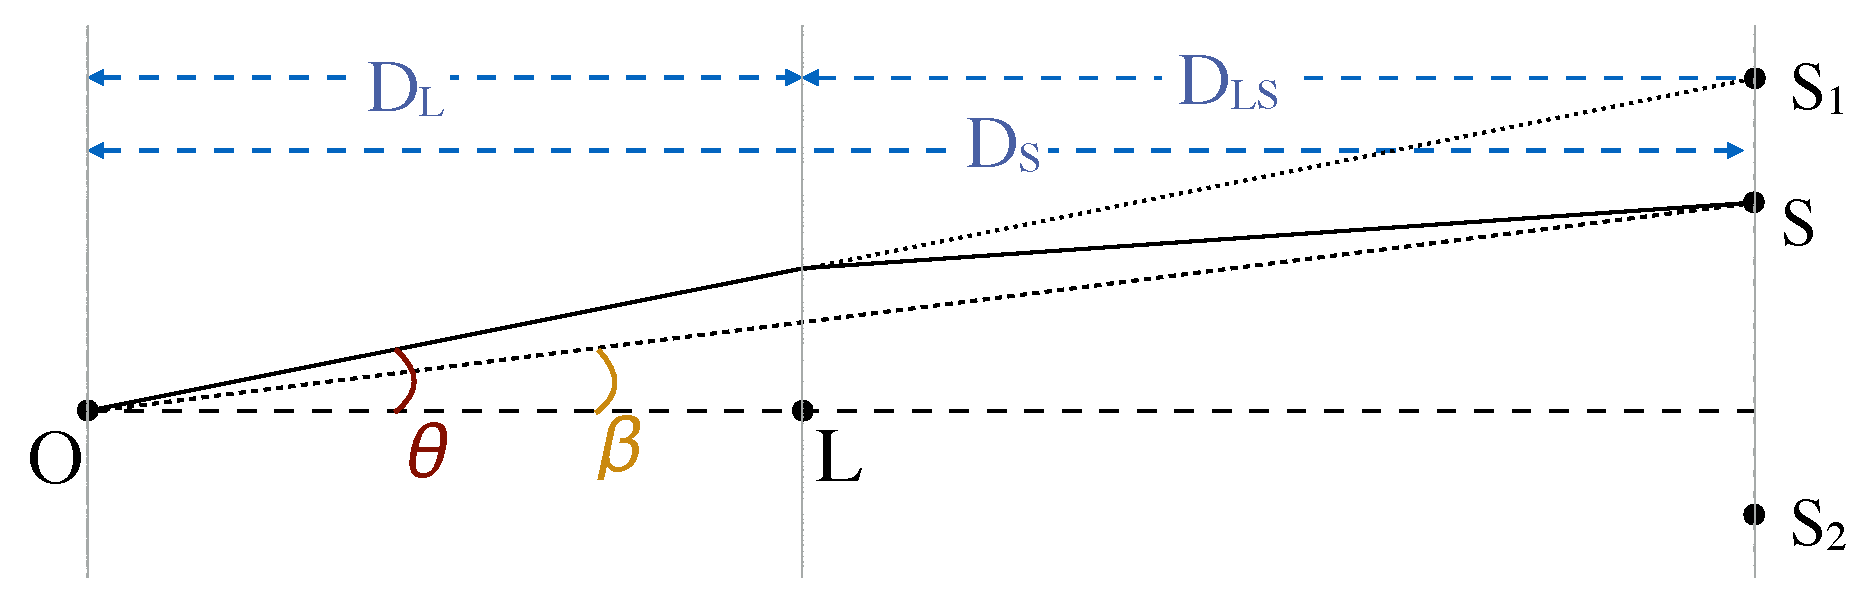
\includegraphics[width=0.5\textwidth]{FIG/lensingGeometry}}
\end{tabular}


\noindent where the redshift of the lens is $z_L$, while \Dl, \Ds, 
and \Dls\ are angular diamater distances from the observer to the
lens, observer to source, and lens to source, respectively.  In the time
delay potential, $\phi$ (Eq.~\ref{eq:phi}), the first term
gives the geometric delay due to light rays following different path
lengths to the observer, and the second term, $\psi$, is the
relativistic component due to differing values of the gravitational
potential along each path.

The distance ratio $\Dl\Ds/\Dls$ in Equation~\ref{eq:dt} is known as
the {\em time delay distance}, and it carries a factor
of \Ho$^{-1}$. Thus, if the lensing potential $\phi$ is well known,
then a time delay measurement provides a direct measurement of the
Hubble constant -- independent of the local distance ladder.  The
distance ratio also has unusual sensitivities to cosmological
parameters as a function of redshift that make this technique a
particularly useful probe of dynamic dark energy
models \citep{Linder:2011}.

\citet{Refsdal:1964} first proposed the use of SN time delays as 
a means to measure \Ho.  Now 50 years later, this has not yet been
achieved, primarily due to the small number of very well analyzed
gravitational lenses ($\sim$dozens), and the short visibility window
for any given high-$z$ SN event ($\sim$a few weeks).  Only recently
have we begun to realize the potential in this technique, with the
measurement of a few dozen time delays of quasars, being lensed
typically by a single foreground galaxy \citep{Jackson:2007}. Among
these, only a handful have time delays measured with particularly high
precision \citep[e.g.][]{Suyu:2010,Suyu:2013}.  These quasar lenses
generally suffer from a number of serious concerns, notably: (1) the
lensing potential is poorly constrained due to inherent degeneracies
and insufficient constraints; (2) the time delays and angular
separations are quite small (tens of days, fractions of an arcsecond);
and (3) the source is continuously variable, often requiring years of
stable monitoring to resolve phase degeneracies.  Wide-field surveys
in the coming decade could deliver $>$100 quasar time delays, but
these problems represent unavoidable systematic biases for this
sample.

\medskip
\noindent {\bf The SN Time Delay Advantage}
 
In Cycle 22, HST has just achieved a new capability for the discovery
of a strongly-lensed SN. The first key advancement was the
availability of WFC3-IR, which allows HST imaging surveys to capture
high-$z$ SN at the peak of their SED profile in rest-frame optical
bands \citep{Rodney:2012,Jones:2013}.  Ground-based surveys and even
HST/ACS programs have searched for multiply-imaged SN in the past, but
none have had the capability to detect even highly magnified SN at
$z>2$ \citep[e.g.][]{Dawson:2009,Sand:2011}.  With WFC3-IR, \Hubble\
now has access to a much larger survey volume with each pointing.

A WFC3-IR program targeting massive clusters, such as CLASH or the
Hubble Frontier Fields, could in principal have caught a strongly
lensed SN already, but in practice the likelihood of such a find was
vanishingly small.  The CLASH team collected WFC3-IR imaging of 25
clusters over 3-years, but the time separation between the first and
last image on any single cluster was typically only a few weeks.
However, these programs -- along with other WFC3-IR cluster imaging
campaigns -- have now provided the second critical advance: deep IR
template imaging of massive clusters from which to construct
difference images for SN discovery.  These HST programs have also led
to an explosion of detailed mass modeling for strong-lensing clusters,
providing well-defined lensing potentials that will be crucial for
evaluating a multiply-imaged SN when one is found.  

Our snapshot program will capitalize on this rich new treasury of IR
cluster imaging in the HST archive, opening the door for a pioneering
time delay distance measurement with the discovery of one or more
strongly lensed SN behind a galaxy cluster.  We will target
well-studied massive clusters that act as especially strong lenses
(Table~\ref{tab:clusters}). For each of these clusters we have dozens
of known multiply-imaged galaxies, and we already have
state-of-the-art lens models in
hand \citep[e.g.][]{Zitrin:2011a,Zitrin:2011b,Zitrin:2012a,Zitrin:2012b,Zitrin:2013}.
Wherever a multiply-imaged SN should appear, {\bf \em we will be
starting out with much better constraints on the lensing potential
$\phi$} than are available for existing quasar time-delay lenses. In
addition to improving the quality of the time-delay cosmography, this
fore-knowledge of the lensing potential will also be crucial for
quickly evaluating any lensed SN candidates we discover, to weed out
impostors before investing precious follow-up time.

Furthermore, {\bf \em the SN we discover behind these clusters will be
inherently better time-delay sources} than the existing sample of
quasars.  Typical time delays through our target clusters are months
or years (not days or weeks as for many lensed quasars), allowing for
more precise measurements of \dt, with ample time to prepare for the
appearance of the second image.  Also, the SN light curve has a single
peak, so there is no possibility of phase ambiguity, and the age of a
SN relative to explosion can be precisely defined from light curve
shape and color, or from spectroscopic
cross-correlation \citep{Filippenko:1997,Blondin:2007}.  Thus the time
delay measurement does not require continuous long-term monitoring,
and can be made with minimal systematic uncertainties.

% Finally, if the SN is of Type Ia (a likely prospect), then light curve
% fitting can provide a luminosity distance measurement with $\sim$8\%
% precision \citep{Phillips:1993}.  Galaxy cluster distances can also be
% estimated using the Sunyaev-Zeldovich effect and x-ray cluster
% luminosities \citep{Silk:1978}.  This means that in addition to the
% time delay distance ratio (\Dl\Ds/\Dls) we can also measure
% independent distances to both the lens and the source.  A \SNIa\ that
% is multiply-imaged by a galaxy cluster would therefore provide a
% unique chance to test for systematic biases in these distance
% estimators.
% %, or even to perform the distance-duality test: if the
% %ratio $\eta_{DD} = D_{S}^{(L)} / ( D_{S}^{(A)}(1+z_S)^2 )$ deviates
% %from unity, then this would signal systematic errors in one or more
% %distances, or a fundamental flaw in the concordance cosmology.


% The large angular separations between our lensed sources and their
% unlensed sight-lines will allow for very precise astrometry that is
% free of systematics due to source blending.  



\medskip
\noindent {\bf The HST Snapshot Search Strategy }

Since Cycle 17, HST surveys of strong lensing clusters (notably CLASH
and the Frontier Fields) have been investing hundreds of orbits in deep
WFC3-IR imaging.  With these templates in hand, the most efficient
way to discover high-$z$ strongly lensed SN is through a relatively
small snapshot program.    To estimate the number of snapshots we
need, we use a tabulation of the number of known multiply-imaged
galaxies in the fields of our target clusters
(Table~\ref{tab:clusters}).  This is a conservative approach, as it is
quite possible to detect a multiply-imaged SN even if the host galaxy
is well below the current detection thresholds for these cluster
fields. The total yield of strongly-lensed SN per snapshot is then

\begin{equation} \label{eq:Nsn}
N_{SN} = SNR_{M} \times M_{gal} \times N_{gal} \times t_{vis},
\end{equation}

\noindent where $SNR_{M^*}$ is the SN rate per unit mass, $M_{gal}$ is
the average mass of a multiply-imaged galaxy, $N_{gal}$ is the number
of multiply imaged galaxies in the field, and $t_{vis}$ is the length
of time that any given SN is visible to our snapshot survey.  Most of
the lensed systems in our target list are at $z\sim 2$, in an era near
the peak of the cosmic star formation history. This should substantially
enhance the rate of both Type Ia and Type II SN, but we conservatively
assume that our average lensed galaxy is generating SN at a rate
similar to an Sb galaxy in our local universe: $SNR_{M} \sim 0.1$ for
both \SNIa\ and SN II \citep{Mannucci:2005}.  We adopt an average
stellar mass of $M_{gal}=10^{10.7} \Msun$ \citep{Tomczak:2013}, and
use the census of multiply-imaged systems in Table~\ref{tab:clusters}
to predict an average of $N_{gal}\sim 35$ lensed galaxy images per
cluster.\footnote{Note that we count each separate image of a
multiple-image set except the last one (typically the most highly
magnified).  The time delay between each image is of order months or
years, so each snapshot is essentially observing the same galaxy at
multiple widely-spaced epochs that can be treated as independent for
the purpose of SN discovery. The last image is not counted because we
can not measure a time delay from the last appearance of a
multiply-imaged SN.}

%\begin{wrapfigure}{r}{0.3\textwidth}
%\minipage[r]{0.29\textwidth}
   
\begin{wraptable}{r}{2.25in}
 \caption{Detection Limits \label{tab:detectionLimits}}
 \begin{tabular}{ccc}
  \toprule
  \toprule
   WFC3/IR & Exp.Time & m$_{lim}$ $^{*}$ \\
   Filter  &  [min] &  [AB mag] \\
   \midrule
   F110W   &    12  &   26.3 \\
   F110W   &    20  &   26.6 \\
   F110W   &    30  &   26.9 \\
   F140W   &    12  &   25.9 \\
   F140W   &    20  &   26.2 \\ 
   F140W   &    30  &   26.5 \\
  \bottomrule
 \multicolumn{3}{p{2.6in}}{$^*$\,Apparent magnitude that yields S/N of 5 (optimum S/N$\sim$10) in the given exposure time.}
\end{tabular}
\end{wraptable}




%\end{minipage}
%\end{wrapfigure}

To maximize the flexibility for scheduling, we consider snapshots with
12, 20 and 30 minutes of exposure time ($\sim$22, 30, and 40 min with
overhead).  These snapshots reach a depth of 25-26 AB mag in the F110W
and F140W filters (Table~\ref{tab:detectionLimits}).  To describe a
realistic distribution of SN visibility times, $t_{vis}$, we use a
census of magnifications and redshifts from all multiply-imaged
galaxies in three of our primary cluster targets
(Figure~\ref{fig:tvis}).  We then use simulated SN light curves to
measure the length of time each SN stays above our detection
threshold, finding an average $t_{vis}\sim 30$ days for \SNIa\ and
$\sim$20 days for SN II.

Inserting these estimates into Eq.~\ref{eq:Nsn}, we find $N_{SN}\sim
0.02$ SN per snapshot, including both Type Ia and II.  To give this
program a realistic chance at discovering a strongly lensed SN in
Cycle 22, we request 200 snapshots, which would yield a sample of
$\sim 4 ^{+3}_{-2}$ SN in one year if all snaps were executed.  With a
realistic snapshot execution rate of $\sim$30\%, that sample drops to
$\sim$one.  These are perilously small sample sizes, but given the
conservative estimates used in this prediction, we expect that a
200-snap allocation will be sufficient to deliver at least one
strongly lensed SN in Cycle 22.  Even just a single detection will
nevertheless be an extraordinary step forward for time delay
cosmography. 

Finally, we note that this snapshot program is designed only for
discovery. Follow-up observations will come from accompanying GO
program, using 12 orbits with ToO observations for immediate
confirmation of a SN candidate and measurement of the light curve.
Sometime in the future, a return campaign to catch the next image
would be needed to complete the time delay measurement, using HST,
ground-based AO systems, or possibly JWST, depending on the length of
the delay.


\medskip
\noindent{\bf Lensed \SNIa\ Probing Cluster Models} 
We could find lensed SN Ia with significant magnification that do not
have multiple images, adding to the sample of SN lensing probes
(Patel+ 2014, Nordin+ 2014).  Classification and light curve
measurement could be done with FrontierSN follow-up orbits


\begin{table}
\caption{Cluster Target List\label{tab:clusters}}
\begin{tabu}{llllcl}
\toprule
\toprule
Cluster & R.A. & Decl. & z & N$_{im}$ $^*$ & References \\
\midrule
\rowfont{\color{blue}}
Abell 2744\dag & 00:14:23.4 & -30:23:26 & 0.31 & 43  & Merten et al. 2011                                         \\
CL0024         & 00:26:35.0 & +17:09:43 & 0.39 & 20  & Zitrin et al. 2009a                                        \\
El Gordo       & 01:02:52.5 & -49:14:58 & 0.87 & 11  & Zitrin et al. 2013b                                        \\
\rowfont{\color{blue}}
Abell 370\dag  & 02:39:52.8 & -01:34:36 & 0.37 & 36  & Richard et al. 2009, ZFF                                   \\
Abell 383      & 02:48:03.4 & -03:31:44 & 0.19 & 18  & Zitrin et al. 2011b                                        \\
\rowfont{\color{blue}}
MACS0416\dag   & 04:16:08.4 & -24:04:21 & 0.40 & 36  & Zitrin et al. 2013                                         \\
MACS0647       & 06:47:50.3 & +70:14:55 & 0.58 & 20  & Zitrin et al. 2011, Coe et al. 2013                        \\
Bullet-a       & 06:58:37.9 & -55:57:00 & 0.3  & 10  & Bradac et al. **                                           \\
Bullet-b       & 06:58:37.9 & -55:57:00 & 0.3  & 11  & Bradac et al. **                                           \\
MACS0717-a     & 07:17:35.6 & +37:44:44 & 0.55 & 18  & Zitrin et al. 2009b, Limousin et al. 2012, Z14             \\
MACS0717-b     & 07:17:35.6 & +37:44:44 & 0.55 & 18  & Zitrin et al. 2009b, Limousin et al. 2012, Z14             \\
MACS0744       & 07:44:52.8 & +39:27:24 & 0.70 & 14  & Zitrin et al. 2011; 2014 in prep                           \\
Abell 611      & 08:00:56.8 & +36:03:23 & 0.21 & 12  & Newman et al. 2013, Z14                                    \\
\rowfont{\color{blue}}
MACS1149\dag   & 11:49:35.7 & +22:23:55 & 0.54 & 29  & Zitrin  \&  Broadhurst 2009, Zheng et al. 2012             \\
\rowfont{\color{blue}}
MACS1206\dag   & 12:06:12.1 & -08:48:04 & 0.44 & 33  & Ebeling et al. 2009, Zitrin et al. 2012                    \\
\rowfont{\color{blue}}
Abell 1689\dag & 13:11:34.2 & -01:21:56 & 0.19 & 117 & Broadhurst et al. 2005, Coe et al. 2010, Diego et al. 2014 \\
\rowfont{\color{blue}}
Abell 1703\dag & 13:15:03.7 & +51:49:27 & 0.28 & 36  & Limousin et al. 200*, Zitrin et al. 2010                   \\
RXJ1347        & 13:47:31.1 & -11:45:12 & 0.45 & 14  & K\"ohlinger \&  Schmidt 2014                               \\
MS1358         & 13:59:48.7 & +62:30:48 & 0.33 & 13  & Zitrin et al. 2011c                                        \\
Abell 1835     & 14:01:02.0 & +02:52:45 & 0.25 & 17  & Richard et al. 2010, Morandi et al. 2012                   \\
Abell 2218     & 16:35:54.0 & +66:13:00 & 0.18 & 18  & Kneib et al. 2004                                          \\
Abell 2261     & 17:22:27.2 & +32:07:57 & 0.22 & 18  & Coe et al. 2012                                            \\
MACS1931       & 19:31:49.6 & -26:34:32 & 0.35 & 10  & Z14                                                        \\
MACS2129       & 21:29:26.1 & -07:41:28 & 0.57 & 14  & Zitrin et al. 2011; Z14                                    \\
\rowfont{\color{blue}}
RXJ2248\dag    & 22:48:44.0 & -44:31:51 & 0.35 & 28  & Monna et al. 2013                                          \\
\bottomrule
% MACS0329   & 03:29:41.6 & -02:11:46 & 0.45 & 11 & Zitrin et al. 2012, Z14                       \\
% MACS0451   & 04:51:54.6 & +00:06:17 & 0.43 & 11                                                 \\
% MACS0454   & 04:54:11.1 & -03:00:53 & 0.54 & 11 & Zitrin et al. 2011                            \\
% CL1226     & 12:26:58.2 & +33:32:48 & 0.89 & 11 & Z14                                           \\
% MACS1423   & 14:23:48.3 & +24:04:47 & 0.54 & 11 & Limousin et al. 2010, Zitrin et al. 2011, Z14 \\
% MACS1720   & 17:20:16.8 & +35:36:26 & 0.39 & 11 & Z14                                           \\
% Abell 2390 & 21:53:55.8 & +17:43:34 & 0.23 & 7  & Frye et al. 1998                              \\
% MS2137     & 21:40:15.2 & -23:39:40 & 0.31 & 7  & Newman et al. 2013, Z14                       \\
% RXJ2129    & 21:29:40.0 & +00:05:21 & 0.23 & 9  & Richard et al. 2010, Z14                      \\
%\enddata
 \multicolumn{6}{p{\textwidth}}{* Approximate number of known strongly-lensed galaxy images
   within the WFC3-IR FOV, counting all instances of each lensed galaxy
   except the last (i.e. all independent lensed galaxy images that
   could deliver a SN time delay measurement).}\\
 \multicolumn{6}{p{\textwidth}}{ \textcolor{blue}{$\dagger$ Primary targets.} We will allocate more
   snapshots to these clusters that have especially strong lenses with
   many multiply-imaged galaxies and particularly good lens models.
   The unweighted average $N_{im}$ is $\sim$25, but we expect this
   weighted snapshot allocation to result in an actual mean of
   $N_{im}\sim 35$.}\\
%\tablenotetext{**}{ Key or latest references for the multiple image
%  compilation in each cluster. Z14 stands for ``Zitrin et al. 2014 in
%  prep" is a soon to be public paper describing our high-end mass
%  models already available online for the community, and multiple
%  images, for all 25 CLASH clusters. ``ZFF" refers to the internal
%  list of the Frontier Fields map making groups, for which Co-PI
%  Zitrin has contributed significantly for revising the multiple
%  images.}
\end{tabu}
\end{table}



\insertfig{FIG/lightcurves.pdf}{ \label{fig:lightcurves} Lensed SN
    light curves }

\insertfig{FIG/tvis_muz_30min.pdf}{\label{fig:tvis} Visibility time
for lensed SN. }






%%%%%%%%%%%%%%%%%%%%%%%%%%%%%%%%%%%%%%%%%%%%%%%%%%%%%%%%%%%%%%%%%%%%%%%%%%%

%   2. DESCRIPTION OF THE OBSERVATIONS
%       (see Section 9.2 of the Call for Proposals)
%
%
\describeobservations   % Do not delete this command.
% Enter your observing description here.
%\begin{wrapfigure}{r}{0.3\textwidth}
%\minipage[r]{0.29\textwidth}
   
\begin{wraptable}{r}{2.25in}
 \caption{Detection Limits \label{tab:detectionLimits}}
 \begin{tabular}{ccc}
  \toprule
  \toprule
   WFC3/IR & Exp.Time & m$_{lim}$ $^{*}$ \\
   Filter  &  [min] &  [AB mag] \\
   \midrule
   F110W   &    12  &   26.3 \\
   F110W   &    20  &   26.6 \\
   F110W   &    30  &   26.9 \\
   F140W   &    12  &   25.9 \\
   F140W   &    20  &   26.2 \\ 
   F140W   &    30  &   26.5 \\
  \bottomrule
 \multicolumn{3}{p{2.6in}}{$^*$\,Apparent magnitude that yields S/N of 5 (optimum S/N$\sim$10) in the given exposure time.}
\end{tabular}
\end{wraptable}




%\end{minipage}
%\end{wrapfigure}

In Cycle 22, HST has just achieved a new capability for the discovery
of a multiply-imaged SN. Three key ingredients will make this program
feasible for the first time in this cycle: (1) the use of
WFC3-IR, (2) a SNAP survey strategy
with repeated shallow visits over many clusters, and (3) a carefully
optimized target list of clusters with both IR template imaging
and excellent mass models.

\noindent {\bf 1. WFC3-IR:~~~} Ground-based surveys and even HST/ACS programs
have looked for lensed
SN \citep[e.g.][]{Sharon:2007,Dawson:2009,Sharon:2010,Sand:2011}, but
none of these have had the capability to detect SN at $z\sim2$, even
with substantial magnification, so many multiply-imaged
galaxies were effectively unreachable to them.
\citet{Amanullah:2011}
demonstrated the value of searching for high-$z$ SN at IR wavelengths,
where one samples rest-frame optical bands at the peak of the SN
SED. Using a K-band survey from the VLT with HAWK-I\footnote{VLT: Very
Large Telescope; HAWK-I: High Acuity Wide-field K-band Imager} they
discovered of a lens-magnified SN at $z\sim1.7$ behind the galaxy
cluster Abell 1689.  With the CANDELS and CLASH programs, we have
taken this IR search strategy above the atmosphere, showing that
WFC3-IR is capable of discovering even un-lensed SNe at
$z>1.5$ \citep{Rodney:2012,Jones:2013}, and finding three more
lens-magnified SNe \citep{Patel:2013,Nordin:2014}.  The ongoing Hubble
Frontier Fields (HFF) program (PI:Lotz) is gathering deep WFC3-IR
imaging of 6 galaxy clusters, and with our multi-cycle GO program
(PI:Rodney) we have already found 8 SN in the HFF data, including 2
with significant magnification.  However, all of these magnified SN
are too far away from the cluster center to be multiply-imaged.

\noindent {\bf 2. Snapshots:~~~} A primary reason that
recent WFC3-IR surveys have not found any multiply-imaged SN is
because they are optimized for depth and wavelength coverage instead
of cadence.  CLASH, for example, collected WFC3-IR imaging of 25
clusters over 3 years, but many orbits were allocated to ACS and
WFC3-UVIS, and the time separation between the first and last IR image
on any single cluster was typically only $\sim$40 days.  Thus, in
practice each cluster only had one epoch suitable for a lensed SN
search, making any detection extremely unlikely.  The HFF program only
exacerbates this problem, by drilling even deeper on a much smaller
number of clusters.  However, CLASH, HFF and other programs have now
provided deep IR template imaging of many massive clusters from which
to construct difference images for SN discovery.

Our snapshot program will capitalize on this rich archival treasury by
delivering hundreds of shallow visits across $\sim$25 clusters. We
will use snapshots with 12, 20 and 30 minutes of total exposure time
to provide maximal flexibility for scheduling.  The stochastic
snapshot scheduling process will typically ensure that our visits are
spread over a long time baseline, maximizing our chance of catching a
new multiply-imaged SN in action.  However, if multiple snapshots on
the same cluster do get scheduled together, then the added depth
simply makes that epoch more sensitive to faint SN.  We will use a mix
of F110W and F140W snapshots so that same-epoch snaps will also
provide some minimal color information that can aid in preliminary SN
classification.  Anticipated detection limits are given in
Table~\ref{tab:detectionLimits}, and Figure~\ref{fig:tvis} shows that
our snaps will be deep enough that \SNIa\ will be visible for long
periods in most of the lensed galaxy images for our sample.


\noindent {\bf 3. Cluster Target Selection:~~~}
The HST archive now holds a deep trove of ACS and (most notably)
WFC3-IR imaging on strong-lensing galaxy clusters at redshifts
$z\sim0.2-0.7$.  This valuable data set has led to an explosion of
high quality cluster lens models, thanks to much effort in
supplemental observations and modeling \citep[e.g.][]{Kneib:2004,
Smith:2005, Limousin:2008, Bradac:2008, Richard:2009}.  Co-PI Zitrin
has had a leading role in this recent burst, principally through the
light-traces-mass (LTM) lens modeling technique, which particularly
excels with its predictive power for the discovery of multiply-imaged
galaxies \citep{Broadhurst:2005, Zitrin:2009a}.  Through the CLASH
program, this approach has been used to generate precise mass models
for a few dozen clusters, dramatically expanding the number of strong
lensing clusters with many known multiple-image
systems \citep[e.g.][]{Zitrin:2009a, Zitrin:2009b, Zitrin:2011a,
Zitrin:2011b, Zitrin:2011c, Merten:2011, Zitrin:2012a, Zitrin:2012b,
Zitrin:2013a, Zitrin:2013b, Coe:2012, Coe:2013}.  The quality of our
lens models will translate directly into the uncertainty in our
determination of \Ho.  We find that reaching $\sim$10\% precision
on \Ho\ is a very plausible benchmark (Figure~\ref{fig:dterr}),
consistent with past
estimates \citep{Bolton:2003,Oguri:2003,Riehm:2011}.

To build our target list, we have taken into account the trade-off
between the number of lensed galaxies and the length of their time
delays.  Very massive clusters will generally provide more
multiply-imaged background galaxies that could host a SN during our
survey.  However, very massive clusters will also on average yield
time delays which are too long to be of practical use hard to measure
on a reasonable time scale (\dt~can be $\sim10^{2-3}$ years). In some
cases only $\sim20\%$ of the multiple-image pairs behind these
monster lenses would yield desirable time delays on the scale of
months to years.  Therefore, the optimal cluster lens targets are
medium-to-large lenses with Einstein radii of roughly
$\sim10-30\arcsec$.  There is also some dependence on the exact
structure and redshift of the lens, but as a rule of thumb such lenses
will each have about $\sim10-40$ multiple galaxy images with useful time
delays.

Table~\ref{tab:clusters} presents our list of 25 cluster targets,
which are spread across the sky to optimize snapshot
observability. The list is dominated by moderate-to-large lenses, but
supplemented with some more massive clusters that contain more
multiple images.


%%%%%%%%%%%%%%%%%%%%%%%%%%%%%%%%%%%%%%%%%%%%%%%%%%%%%%%%%%%%%%%%%%%%%%%%%%%

%   3. SPECIAL REQUIREMENTS
%       (see Section 9.3 of the Call for Proposals)
%
%
\specialreq             % Do not delete this command.
% Justify your special requirements here, if any.
This snapshot program is designed exclusively for SN
discovery. Follow-up observations will come from an accompanying GO
program (PI: Strolger), which should be evaluated in concert with this
proposal.



%%%%%%%%%%%%%%%%%%%%%%%%%%%%%%%%%%%%%%%%%%%%%%%%%%%%%%%%%%%%%%%%%%%%%%%%%%%

%   4. COORDINATED OBSERVATIONS
%       (see Section 9.4 of the Call for Proposals)
%
%
%\coordinatedobs          % Do not delete this command.
% Enter your coordinated observing plans here, if any.
%\input{coordinatedobs}

%%%%%%%%%%%%%%%%%%%%%%%%%%%%%%%%%%%%%%%%%%%%%%%%%%%%%%%%%%%%%%%%%%%%%%%%%%%

%   5. JUSTIFY DUPLICATIONS
%       (see Section 9.5 of the Call for Proposals)
%
%
\duplications           % Do not delete this command.
% Enter your duplication justifications here, if any.
This program necessarily re-visits fields with substantial HST
imaging. We rely on the existing WFC3-IR data to provide template
imaging for SN discovery.  



%%%%%%%%%%%%%%%%%%%%%%%%%%%%%%%%%%%%%%%%%%%%%%%%%%%%%%%%%%%%%%%%%%%%%%%%%%%
%  Bibliography goes in before or after PAST HST usage ??
%  Probably before, since it has to be counted in the text page limit
%%%%%%%%%%%%%%%%%%%%%%%%%%%%%%%%%%%%%%%%%%%%%%%%%%%%%%%%%%%%%%%%%%%%%%%%%%%

%\smallskip
\newpage
\setlength{\bibsep}{-2pt}
\begin{spacing}{0.5}
\bibliographystyle{apjbrief}
{\footnotesize
\bibliography{bibdesk}
}
\end{spacing}



%%%%%%%%%%%%%%%%%%%%%%%%%%%%%%%%%%%%%%%%%%%%%%%%%%%%%%%%%%%%%%%%%%%%%%%%%%%

%   7. FIGURES AND TABLES  (must appear after the text)
\clearpage


\begin{SCfigure}
  \centering
  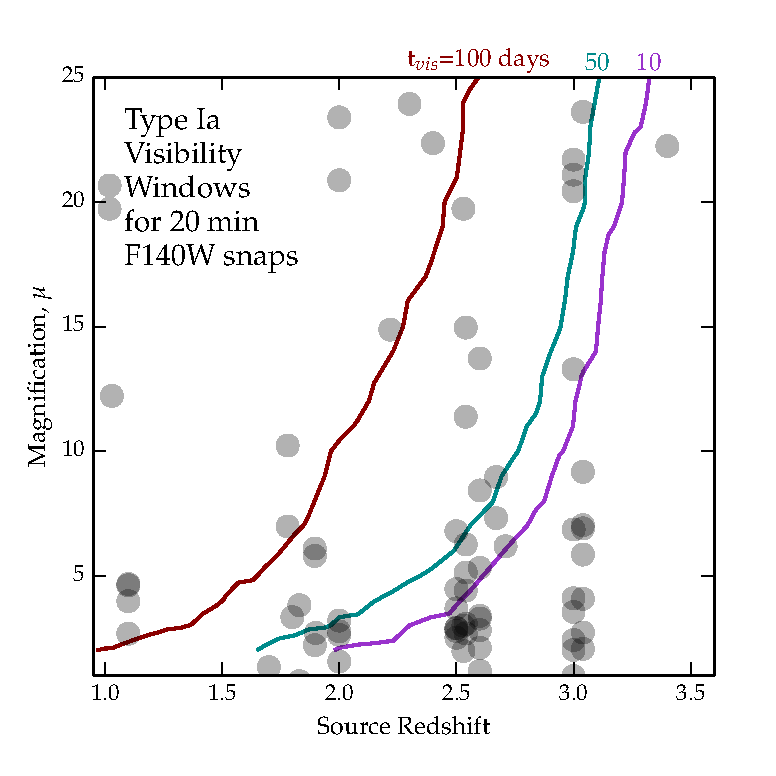
\includegraphics[width=0.5\textwidth]{FIG/tvis_muz_20min.pdf}
  \caption{ \label{fig:tvis}
Visibility time contours in the redshift-magnification plane.  For any
given redshift and magnification, we estimate $t_{vis}$, the number of
days that an average \SNIa\ would be detectable in a 20-minute
snapshot.  Solid lines plot contours of constant visibility time in
the $z-\mu$ plane at $t_{vis}=$100, 50, and 10 days.  Grey circles
mark the magnifications and redshifts for 50 strongly-lensed galaxy
images from three of our primary cluster targets.  Thus, if a galaxy
lies to the left of the 50-day line, then it is visible to our survey
for at least 50 days. }
\end{SCfigure}


\begin{figure}
  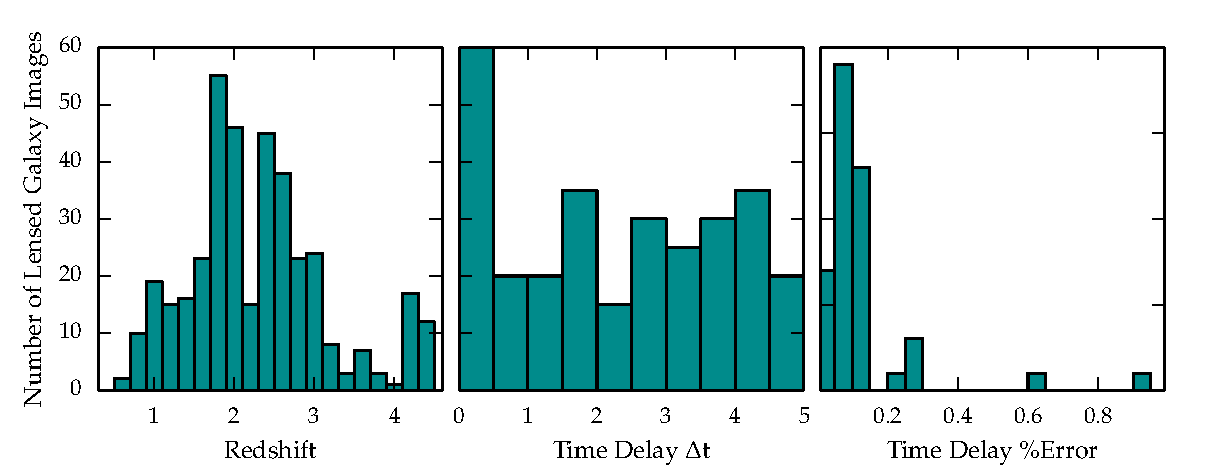
\includegraphics[width=\textwidth]{FIG/histograms.pdf}
  \caption{ \label{fig:tvis} Histograms showing the distribution of a
    representative sample of lensed galaxy images over redshift
    (left), time delay (middle) and time delay precision (right). 
}
\end{figure}




%%%%%%%%%%%%%%%%%%%%%%%%%%%%%%%%%%%%%%%%%%%%%%%%%%%%%%%%%%%%%%%%%%%%%%%%%%%

%   6. PAST HST USAGE
%       (see Section 9.8 of the Call for Proposals)
%
%        List here the program numbers and data status for all accepted GO/AR/SNAP 
%        programs of the PI in at least the last four HST Cycles. Include a list of refereed publications 
%        resulting from these programs.       
%
%       Note that the description of past HST usage  DOES NOT count against the page limits of the proposal.
%

%\pagebreak
\newpage
\pasthstusage  % Do not delete this command.

% all accepted GO/AR/SNAP Programs of the PI in the last four HST cycles.

Table\,\ref{tab:pasthstusage} lists the HST programs from recent cycles that include PI Rodney.

% \begin{deluxetable}{p{0.25\linewidth}p{0.15\linewidth}p{0.2\linewidth}p{0.3\linewidth}}
% %\rotate
% \tablecolumns{4}
% \tablecaption{Past HST Usage for PI \label{tab:pasthstusage}}
% \tablehead{   \colhead{PID}  & \colhead{Title} & \colhead{Status} & 
%   \colhead{Selected Publications\tablenotemark{*}} }
% \startdata
% 12060-64, 12440-45 & CANDELS & Cycle 18-20 MCT;\linebreak $\sim$90\% complete. & \citealt{Grogin:2011}\linebreak \citealt{Trump:2011}\linebreak \citealt{van-der-Wel:2011} \\[6pt]
% 12065-69, 12100-04, 12451-60 & CLASH & Cycle 18-20 MCT;\linebreak $\sim$90\% complete. & \citealt{Postman:2012}\linebreak \citealt{Coe:2013}\\[22pt]
% 12099, 12461, 13063 & C+C SN Follow-up & Cycle 18-20 MCT;\linebreak $\sim$90\% complete. & \citealt{Rodney:2012}\linebreak \citealt{Frederiksen:2012}\linebreak \citealp{Jones:2013}\\[6pt]
% 13046 & RAISIN & Cycle 20 ToO;\linebreak collecting data & \nodata \\
% \enddata
% \tablenotetext{*}{Listed publications are those with direct input from PI Rodney and the CANDELS+CLASH SN team. Total CANDELS+CLASH publications $\approx$63.}
% \end{deluxetable}






\end{document}          % End of proposal. Do not delete this line.
                        % Everything after this command is ignored.

